%==============================================================
%  EE201  Circuit Theory I  --  Fall 2026/27
%  Syllabus presented as slides (first lecture, piece by piece)
%  Section 2 -- Mert Ankarali
%
%  Compile:  pdflatex 2026_Syllabus_slides.tex   (twice)
%  Uses only standard beamer -- no external theme package needed.
%==============================================================
\documentclass[11pt,aspectratio=169]{beamer}

\usepackage[T1]{fontenc}
\usepackage[utf8]{inputenc}
\usepackage[english]{babel}
\usepackage{lmodern}
\usepackage{booktabs}
\usepackage{array}
\usepackage{tikz}
\usepackage{colortbl}

%-------------------- a plain METU-flavoured theme ------------
\usetheme{default}
\usecolortheme{default}
\useinnertheme{rectangles}
\setbeamertemplate{navigation symbols}{}
\setbeamertemplate{itemize items}[square]
\setbeamertemplate{enumerate items}[default]
\setbeamerfont{frametitle}{size=\large,series=\bfseries}
\setbeamerfont{title}{size=\LARGE,series=\bfseries}

\definecolor{metured}{RGB}{155,27,48}
\definecolor{metugray}{RGB}{88,89,91}
\definecolor{metulight}{RGB}{243,240,241}

\setbeamercolor{structure}{fg=metured}
\setbeamercolor{frametitle}{fg=metured,bg=}
\setbeamercolor{title}{fg=metured}
\setbeamercolor{normal text}{fg=black!88}
\setbeamercolor{block title}{fg=white,bg=metured}
\setbeamercolor{block body}{bg=metulight}
\setbeamercolor{alerted text}{fg=metured}

% frame title with a thin rule underneath
\setbeamertemplate{frametitle}{%
  \vspace{0.6em}%
  \usebeamerfont{frametitle}\usebeamercolor[fg]{frametitle}\insertframetitle\par
  \vspace{-0.2em}{\color{metured}\rule{\textwidth}{1pt}}\par\vspace{-0.2em}}

% footline: course - term - section - page
\setbeamertemplate{footline}{%
  \hbox{\begin{beamercolorbox}[wd=\paperwidth,ht=2.4ex,dp=1.4ex,leftskip=1.2em,rightskip=1.2em]{}%
  \tiny\color{metugray}\coursecode\ \coursename\ \textbar\ \term\ \textbar\ \mysection\
  \hfill \insertframenumber/\inserttotalframenumber
  \end{beamercolorbox}}}

%-------------------- macros (keep in sync with the syllabus) --
\newcommand{\coursecode}{EE201}
\newcommand{\coursename}{Circuit Theory I}
\newcommand{\term}{Fall 2026--2027}
\newcommand{\mysection}{Section 2}
\newcommand{\myname}{Mert Ankaralı}
\newcommand{\myoffice}{A-410/D-104}
\newcommand{\mymail}{mertan@metu.edu.tr}
% >>> Public repository that hosts the lecture notes of Section 2 <<<
% Repo: mertankarali/Lecture-Notes (public), course folder: METU-EE201
\newcommand{\notesrepo}{https://github.com/mertankarali/Lecture-Notes/tree/master/METU-EE201}
\newcommand{\notesrepotext}{github.com/mertankarali/Lecture-Notes}
\newcommand{\odtuclass}{https://odtuclass.metu.edu.tr}
\newcommand{\coordinator}{Prof. T. Engin Tuncer}
\newcommand{\coordinatormail}{etuncer@metu.edu.tr}
\newcommand{\tunanotes}{https://users.metu.edu.tr/etuna/ee201/}
\newcommand{\tunanotestext}{users.metu.edu.tr/etuna/ee201}

\hypersetup{colorlinks=true,allcolors=metured}

\newcolumntype{L}[1]{>{\raggedright\arraybackslash}p{#1}}

\title{\coursecode: \coursename}
\subtitle{Syllabus --- \term}
\author{\myname\ \\ \small \mysection}
\institute{\small Department of Electrical and Electronics Engineering\\ Middle East Technical University}
\date{}

%==============================================================
\begin{document}

%--------------------------------------------------------------
\begin{frame}[plain]
  \titlepage
  \begin{center}
    \small\color{metugray}
    Section 2 material: \href{\notesrepo}{\ttfamily \notesrepotext}
  \end{center}
\end{frame}

%==============================================================
\section{People}
%--------------------------------------------------------------
\begin{frame}{Instructors --- \coursecode, \term}
  \begin{center}
  \small
  \begin{tabular}{c L{4.2cm} c L{4.6cm}}
    \toprule
    \textbf{Section} & \textbf{Instructor} & \textbf{Office} & \textbf{e-mail}\\
    \midrule
    1 & T. Engin Tuncer & E109  & etuncer@metu.edu.tr\\
    \rowcolor{metulight}
    \textbf{2} & \textbf{\myname} & \textbf{\myoffice} & \textbf{\mymail}\\
    3 & Emre Tuna   & E113  & etuna@metu.edu.tr\\
    4 & Emre Tuna   & E113  & etuna@metu.edu.tr\\
    5 & Yunus Aslan & C-103 & aslany@metu.edu.tr\\
    \bottomrule
  \end{tabular}
  \end{center}
  \vfill
  \centering\small\color{metugray}
  You are in \textbf{\mysection} --- office \myoffice, \mymail
\end{frame}

%--------------------------------------------------------------
\begin{frame}{Teaching assistants}
  \begin{block}{\coursecode\ --- theory}
    Anıl Gülbeden \hfill \texttt{gulbeden@metu.edu.tr}
  \end{block}
  \begin{block}{\coursecode/EE213 --- laboratory}
    Alp Gürsoy \quad Eda Özkaynar \quad Orhun Koç \quad Civan Serhat Çevik\\
    Elif Çağla Tay \quad Enfal Çabuk \quad Adem Utku Atasayar\\
    Özgür Gülsuna \quad Alper Alka
  \end{block}
  \vfill
  \small Laboratory questions go to the laboratory assistants first;
  theory questions to the course assistant or the instructors.
\end{frame}

%==============================================================
\section{Material}
%--------------------------------------------------------------
\begin{frame}{Course material --- common to all sections}
  \begin{enumerate}
    \item \textbf{Alexander \& Sadiku}, \emph{Fundamentals of Electric Circuits},
          McGraw-Hill, 2016. \hfill \alert{main textbook}
    \item \textbf{Chua, Desoer \& Kuh}, \emph{Linear and Nonlinear Circuits},
          McGraw-Hill, 1987. \hfill reference
    \item Lecture notes and videos by \textbf{Emre Tuna} ---
          \href{\tunanotes}{\texttt{\tunanotestext}}
  \end{enumerate}
  \vfill
  \begin{block}{ODTÜCLASS --- \href{\odtuclass}{odtuclass.metu.edu.tr}}
    The official channel for \emph{all} sections: announcements, the detailed course outline,
    grades, exam and laboratory information, and the common material above.
  \end{block}
  \vfill
  \centering\small\color{metugray}
  Reading the textbook \emph{before} the lecture is worth more than reading it after.
\end{frame}

%--------------------------------------------------------------
\begin{frame}{And, for \mysection: a course repository}
  \vfill
  \begin{center}
    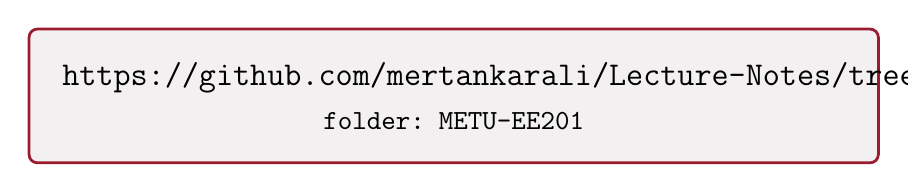
\begin{tikzpicture}
      \node[draw=metured,line width=1pt,fill=metulight,rounded corners=3pt,
            inner sep=12pt,text width=0.82\textwidth,align=center]
      {\large\ttfamily \href{\notesrepo}{\notesrepotext}\\[4pt]\normalsize folder: METU-EE201};
    \end{tikzpicture}
  \end{center}
  \vfill
  \begin{itemize}
    \item My lecture notes and supplementary material for this section.
    \item \textbf{Public} --- no account needed to read or download.
    \item Updated \textbf{during} the semester, usually before each lecture.
    \item Clone it and \texttt{git pull}, or just re-download --- but do not work from a copy
          you downloaded in October.
    \item Found a typo or an error? Open an issue or send me an e-mail.
  \end{itemize}
\end{frame}

%--------------------------------------------------------------
\begin{frame}{What is where}
  \begin{columns}[T,onlytextwidth]
    \column{0.48\textwidth}
      \begin{block}{ODTÜCLASS (all sections)}
        \small
        \begin{itemize}
          \item official announcements
          \item detailed course outline
          \item grades
          \item exam and laboratory info
          \item common notes and videos
        \end{itemize}
      \end{block}
    \column{0.48\textwidth}
      \begin{block}{Repository (\mysection)}
        \small
        \begin{itemize}
          \item my lecture notes
          \item supplementary material
        \end{itemize}
      \end{block}
  \end{columns}
  \vfill
  \centering\small\color{metugray}
  Announcements are \emph{always} on ODTÜCLASS. The repository is for content.
\end{frame}

%==============================================================
\section{Grading and rules}
%--------------------------------------------------------------
\begin{frame}{Grading}
  \begin{center}
  \begin{tabular}{L{6cm} r}
    \toprule
    \textbf{Component} & \textbf{Weight}\\
    \midrule
    Attendance       & 5\,\%\\
    Midterm Exam 1   & 20\,\%\\
    Midterm Exam 2   & 20\,\%\\
    Final Exam       & 35\,\%\\
    Laboratory       & 20\,\%\\
    \midrule
    \textbf{Total}   & \textbf{100\,\%}\\
    \bottomrule
  \end{tabular}
  \end{center}
  \vfill
  \centering\small\color{metugray}
  The laboratory is one fifth of your grade --- and a gate, see the next slide.
\end{frame}

%--------------------------------------------------------------
\begin{frame}{Attendance in \mysection}
  \begin{itemize}
    \item Taken with a \alert{QR code on ODTÜCLASS} --- bring a device that can read it.
    \item \textbf{Once per class meeting} --- once in a one-hour meeting, once in a two-hour
          meeting. Not once per lecture hour.
    \item Normally \textbf{at the beginning}. In a two-hour meeting, if I give a break,
          I may open it \textbf{at the break} instead.
    \item I sometimes teach two hours as one block, sometimes finish early, and I do not
          always open it at the break.
  \end{itemize}
  \vfill
  \begin{block}{So}
    There is no pattern to rely on. Skipping the first hour and arriving at the break is
    \alert{your own risk} --- if attendance was taken while you were not in the room,
    that meeting is lost and it is not repeated.
  \end{block}
\end{frame}

%--------------------------------------------------------------
\begin{frame}{Final examination policy --- how to get an NA}
  You will \alert{not be admitted to the final exam} and will receive \alert{NA} if:
  \vspace{0.6em}
  \begin{enumerate}
    \item your attendance is below \textbf{40\,\%};
    \item you miss \textbf{any midterm} without a valid excuse;
    \item you miss \textbf{any laboratory experiment} without a valid excuse;
    \item you miss the \textbf{Laboratory Final Exam} without a valid excuse.
  \end{enumerate}
  \vfill
  \begin{block}{Read this as}
    Show up, and if something happens, report it \emph{with a valid excuse and on time}.
  \end{block}
\end{frame}

%--------------------------------------------------------------
\begin{frame}{Make-up policy}
  \begin{itemize}
    \item A make-up compensates for \textbf{one} missing exam or laboratory.
    \item Missing more than one $\Rightarrow$ multiple make-ups.
    \item Make-ups may be scheduled \textbf{before or after} the final exam.
    \item Dates are announced on \href{\odtuclass}{ODTÜCLASS};
          the laboratory make-up is announced \textbf{separately}.
  \end{itemize}
  \vfill
  \centering\small\color{metugray}
  Follow the ODTÜCLASS announcements --- "I did not know" is not an excuse.
\end{frame}

%--------------------------------------------------------------
\begin{frame}{If you have taken EE213 or the old \coursecode}
  \begin{itemize}
    \item \textbf{Took EE213, have a grade, now registered to the new \coursecode:}\\
          your grade comes from the \coursecode\ \emph{theoretical} part (100\,\%);
          the previous laboratory grade is \textbf{not} included.
    \item \textbf{Failed EE213 and take only the EE213 laboratory:}\\
          your grade comes from the laboratory work only, as before.
    \item \textbf{New \coursecode\ (theory + laboratory)} is opened only for students
          taking the course for the \textbf{first time}.
  \end{itemize}
  \vfill
  \centering\small\color{metugray}
  Unsure which case you are in? Send an e-mail to the course coordinator,
  \coordinator\ (\texttt{\coordinatormail}).
\end{frame}

%==============================================================
\section{Content}
%--------------------------------------------------------------
\begin{frame}{Course outline --- the whole semester}
  \begin{center}
  \small
  \begin{tabular}{L{8.4cm} r}
    \toprule
    \textbf{Topic} & \textbf{Hours}\\
    \midrule
    1. Basic Concepts                          & 6\\
    2. Linear Time-Invariant Resistive Circuits & 10\\
    3. Nonlinear Resistive Circuits             & 3\\
    4. Operational Amplifier Circuits           & 7\\
    5. Dynamic Elements                         & 5\\
    6. First Order Circuits                     & 11\\
    \midrule
    \textbf{Total}                              & \textbf{42}\\
    \bottomrule
  \end{tabular}
  \end{center}
  \vfill
  \centering\small\color{metugray}
  Next three slides: what is inside each of these.
\end{frame}

%--------------------------------------------------------------
\begin{frame}{Outline (1/3) --- resistive circuits}
  \begin{block}{1. Basic Concepts \hfill 6 hrs}
    Introduction; lumped elements and lumped circuits; interconnection equations;
    branch relations; basic lumped elements; circuit analysis.
  \end{block}
  \begin{block}{2. Linear Time-Invariant Resistive Circuits \hfill 10 hrs}
    LTI resistive elements: resistors, dependent sources, ideal transformers;
    analysis methods; one-port circuits; two-ports.
  \end{block}
  \vfill
  \centering\small\color{metugray}
  This is where the language of the course is built --- do not fall behind here.
\end{frame}

%--------------------------------------------------------------
\begin{frame}{Outline (2/3) --- nonlinearity and op-amps}
  \begin{block}{3. Nonlinear Resistive Circuits \hfill 3 hrs}
    Nonlinear resistive elements and circuits; load-line analysis;
    piecewise-linear resistive circuits.
  \end{block}
  \begin{block}{4. Operational Amplifier Circuits \hfill 7 hrs}
    Operational amplifiers; basic op-amp circuits; more realistic op-amp models;
    miscellaneous resistive op-amp circuits; op-amps with piecewise-linear elements.
  \end{block}
\end{frame}

%--------------------------------------------------------------
\begin{frame}{Outline (3/3) --- dynamics}
  \begin{block}{5. Dynamic Elements \hfill 5 hrs}
    Ramp, step and impulse functions; capacitors; inductors.
  \end{block}
  \begin{block}{6. First Order Circuits \hfill 11 hrs}
    First order linear ODEs with constant coefficients; simple LTI RC circuit;
    simple LTI RL circuit; miscellaneous LTI first order circuits;
    piecewise-linear first order circuits.
  \end{block}
  \vfill
  \centering\small\color{metugray}
  From algebraic equations to differential equations --- the heart of the course.
\end{frame}

%--------------------------------------------------------------
\begin{frame}{Laboratory outline}
  \begin{center}
  \begin{tabular}{l L{8.6cm}}
    \toprule
    \textbf{Exp.} & \textbf{Title}\\
    \midrule
    \#1 & Introduction to Voltage, Current and Resistance Measurements\\
    \#2 & Signal Generators and Oscilloscopes\\
    \#3 & LTspice Workshop \textit{(computer experiment)}\\
    \#4 & Resistive Circuits\\
    \#5 & Operational Amplifiers\\
    \#6 & First Order Circuits\\
    \bottomrule
  \end{tabular}
  \end{center}
  \vfill
  \centering\small\color{metugray}
  The experiments follow the theory --- and missing one without an excuse means NA.
\end{frame}

%==============================================================
%--------------------------------------------------------------
\begin{frame}{Before the next lecture}
  \begin{enumerate}
    \item Check that you are enrolled on \href{\odtuclass}{ODTÜCLASS} for \coursecode\
          --- and for EE213 as well, if you take the laboratory separately.
    \item Open the repository and bookmark it:\\[2pt]
          \hspace*{1.2em}\ttfamily \href{\notesrepo}{\notesrepotext}
    \item Get the textbook (Alexander \& Sadiku) and skim Chapter 1.
    \item Note the detailed outline on ODTÜCLASS.
  \end{enumerate}
  \vfill
  \begin{center}
    \Large\color{metured}\textbf{Questions?}\\[4pt]
    \normalsize\color{metugray} \myname\ --- \myoffice\ --- \mymail
  \end{center}
\end{frame}

\end{document}
